\newpage
\section{Experiment 4 - Multiobjective EA}
\label{sec:exp4}
In this experiment set the three versions of the Evo-RoleMiner$M$ are tested.

To counteract on the diversity problem and the strong bias of the complexity measure (role count, assignments counts) in the previous experiments, the Evo-RoleMiner$M$ is tested on the Dataset1 (Experiment 4a and 4b) and the Healthcare dataset (Experiment 4c and 4d). For the objectives "Minimizing Confidentiality Violations" and "Minimizing Availability Violations" are chosen, since as shown in Experiment 1 the objectives are conflicting (see section \ref{sec:exp1}). The setup can be seen in Table \ref{tab:exp4_setup}.

\begin{table}[H]
	\centering
	\begin{adjustbox}{width=0.5\textwidth}
		\begin{tabular}{|l|l|}
			\hline
			\rowcolor{myGray} 
			\textbf{Parameter}              & \textbf{Value}    \\ \hline
			Generations                     & 100 / 1000       	\\ \hline
			Population                      & 1000        		\\ \hline
			CXPB                            & 0.25              \\ \hline
			MUTPB-Type1: Add role           & 0.25              \\ \hline
			MUTPB-Type2: Add User           & 0.25              \\ \hline
			MUTPB-Type3: Add Permission     & 0.25              \\ \hline
			MUTPB-Type4: Remove Role        & 0.25              \\ \hline
			MUTPB-Type5: Remove User        & 0.25              \\ \hline
			MUTPB-Type6: Remove Permission  & 0.25              \\ \hline
			Local optimization              & True        		\\ \hline
			Objective 1					    & Confidentiality   \\ \hline
			Objective 2					    & Availability     	\\ \hline
		\end{tabular}
	\end{adjustbox}
	\caption{EXPERIMENT 4 setup. For experiments 4a-b a generation limit of 100 is chosen, while for experiments 4c-d the generation limit is 1000.}
	\label{tab:exp4_setup}
\end{table}

The results are listed in experiment 4a and 4c in Table \ref{tab:exp4_results}. Figure \ref{fig:exp4a_fitness} shows the development of the population in one of the experiments with Dataset1 (for the Healthcare dataset see Appendix \ref{sec:A_Exp4c_Diagrams}). It can be seen that the individuals in each generation have a wide spread and converging near a pareto front. Since the Dataset1 yields a solution where both objectives can be met, the pareto front consist of one point at (0,0) if the solution is found. The objectives of confidentiality and availability violations are only conflicting until the solution is found.

\begin{table}[H]
	\centering
	\caption{Evo-RoleMiner$M$: Results of ten experiments for Dataset1 and Healthcare dataset. The values for each objectives' Fitness, Confidentiality violations ($|G_{conf}|$), Availability violations ($|G_{accs}|$), Roles ($|R|$), User-Role-Assignments ($|UA|$) and Role-Permission assignments ($|RP|$) are the average minimum in the last Generation of the experiments. The values for Interpretability (INT) are the average maximum in the last Generation of the experiments. The generation ($\gamma$), where an individual occurs the first time, which has no violations, is the average out of the ten experiments. The time is the average runtime in seconds.}
	\label{tab:exp4_results}
	\subcaption*{DATASET1}
	\begin{adjustbox}{width=\textwidth}
		\begin{tabular}{|l|l|l|l|c|c|c|c|c|c|c|c|}
			\hline
			\rowcolor{myGray} 
			\textbf{Exp.} & \textbf{Algorithm} & \textbf{Objectives} & \textbf{Fitness} & $\gamma$ & \textbf{$|G_{conf}|$} & \textbf{$|G_{accs}|$} & \textbf{$|R|$} & \textbf{$|UA|$} & \textbf{$|RP|$} & \textbf{INT} & \textbf{Time (in sec)}\\ \hline
			4a & NSGA-II & Conf,Accs &  [0,0] &  53 & 0   &   0 & 4   &   11.1   &   13   &   1    & 156\\ \hline
			4b & NSGA-II$R$ & Conf,Accs &   [0,0] &   23.4 &0   &   0 & 4   &   11.2   &   13.4   &   1    & 256\\ \hline
			4e & NSGA-II$R$ with weights & Viol.,$|UA+PA|$ &   [0,24.7] &   26.2 &   0 & 0 &4   &   13   &   12   &   1    & 139\\ \hline			
		\end{tabular}
	\end{adjustbox}
	\subcaption*{HEALTHCARE}
	\begin{adjustbox}{width=\textwidth}
		\begin{tabular}{|l|l|l|l|c|c|c|c|c|c|c|c|}
			\hline
			\rowcolor{myGray} 
			\textbf{Exp.} & \textbf{Algorithm} & \textbf{Objectives} & \textbf{Fitness} & $\gamma$ & \textbf{$|G_{conf}|$} & \textbf{$|G_{accs}|$} & \textbf{$|R|$} & \textbf{$|UA|$} & \textbf{$|RP|$} & \textbf{INT} & \textbf{Time (in sec)}\\ \hline
			4c & NSGA-II & Conf,Accs &   [0,0] &   $>$1000 &0   &   0 & 17   &   218.6   &   265.8   &   -    & 4076\\ \hline
			4d & \hl{NSGA-II$R$} & Conf,Accs   & [0,0] &   $>$1000 &   0   &   0 & 0   &   0   &   0   &   -    & 0\\ \hline
			4f & \hl{NSGA-II$R$ with weights} & Viol.,$|UA+PA|$ & [0,0] &   $>$1000 &   0   &   0 & 0   &   0   &   0   &   -    & 0\\ \hline		
		\end{tabular}
	\end{adjustbox}
\end{table}
\newpage
\begin{figure}[H]
	\centering
	\begin{subfigure}{\textwidth}
		\centering
		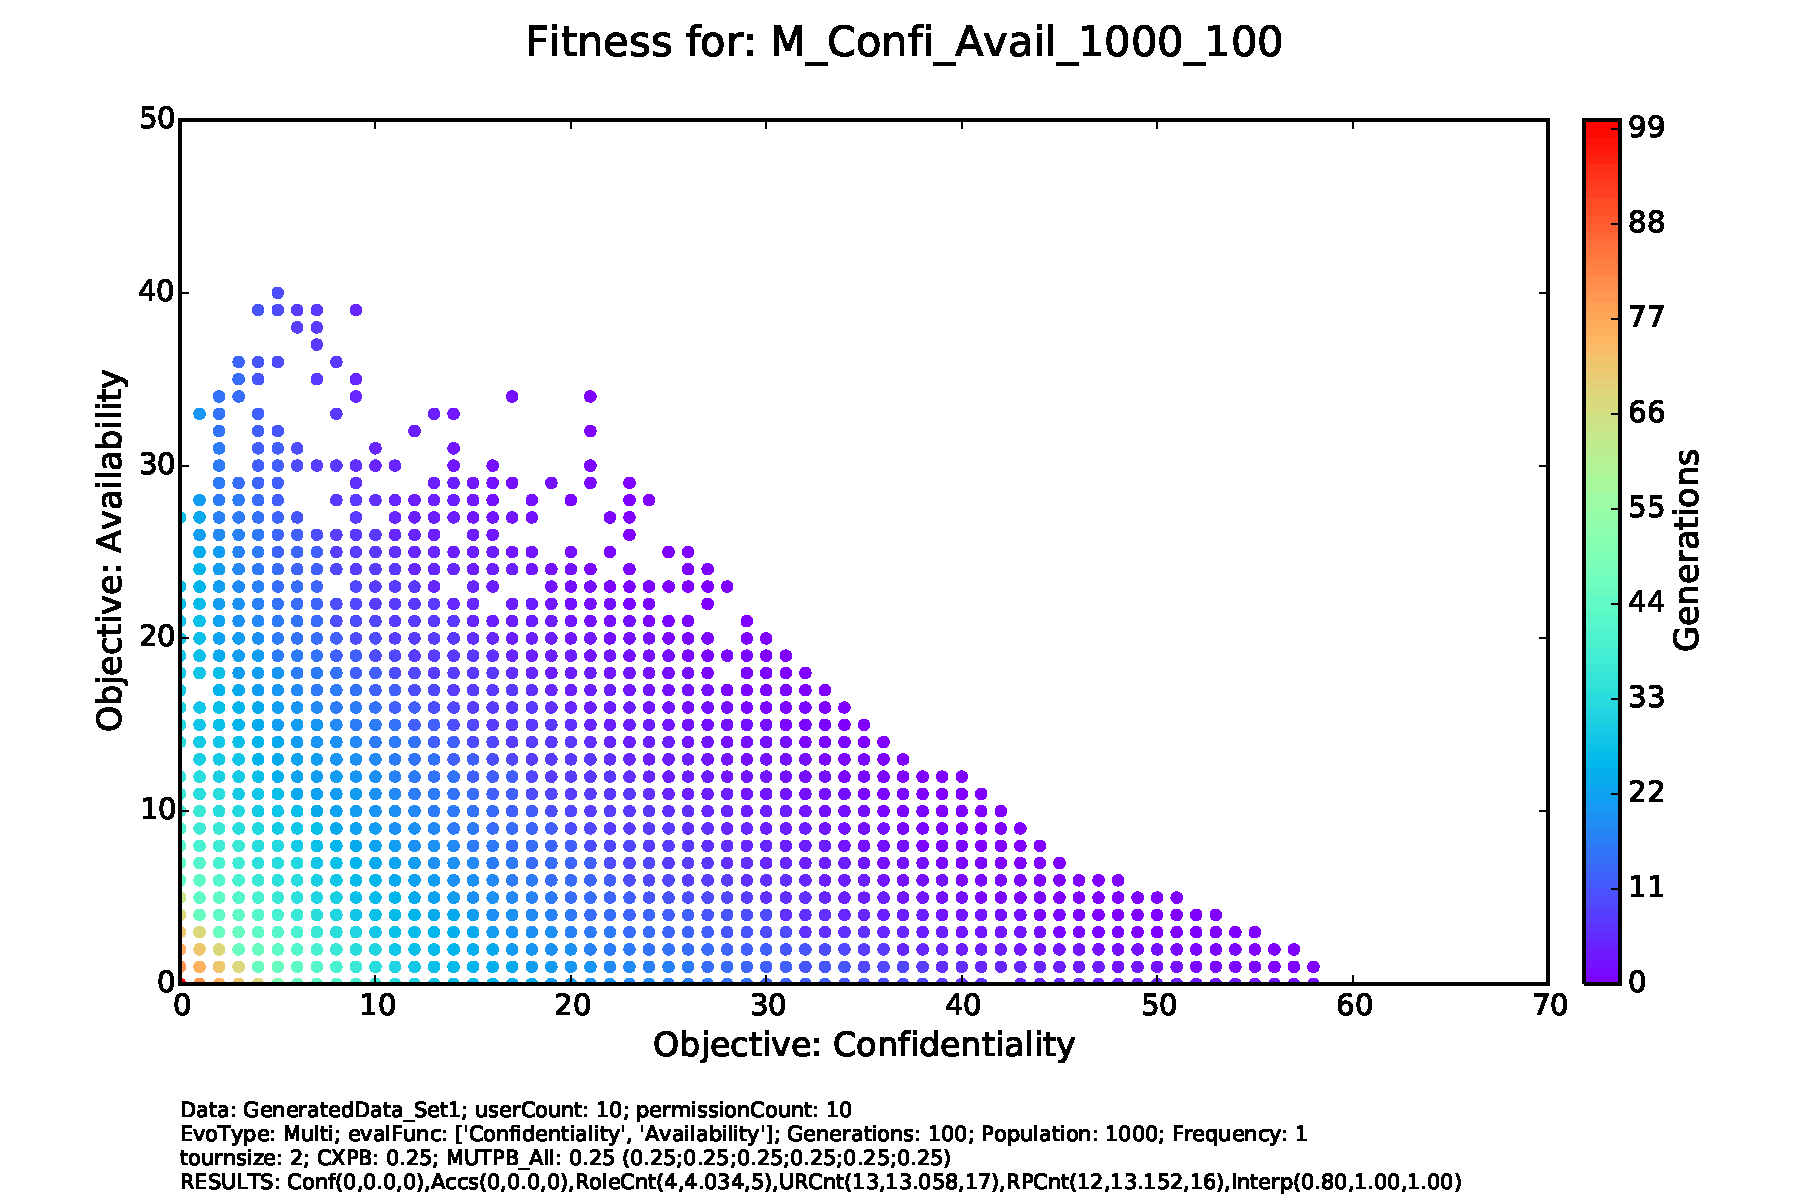
\includegraphics[width=0.8\textwidth, trim=0cm 2cm 0cm 1.5cm, clip=true]{exp4a_fitness}
		\caption{}
		\label{fig:exp4a_fitness_A}
	\end{subfigure}
	\begin{subfigure}{\textwidth}
		\centering
		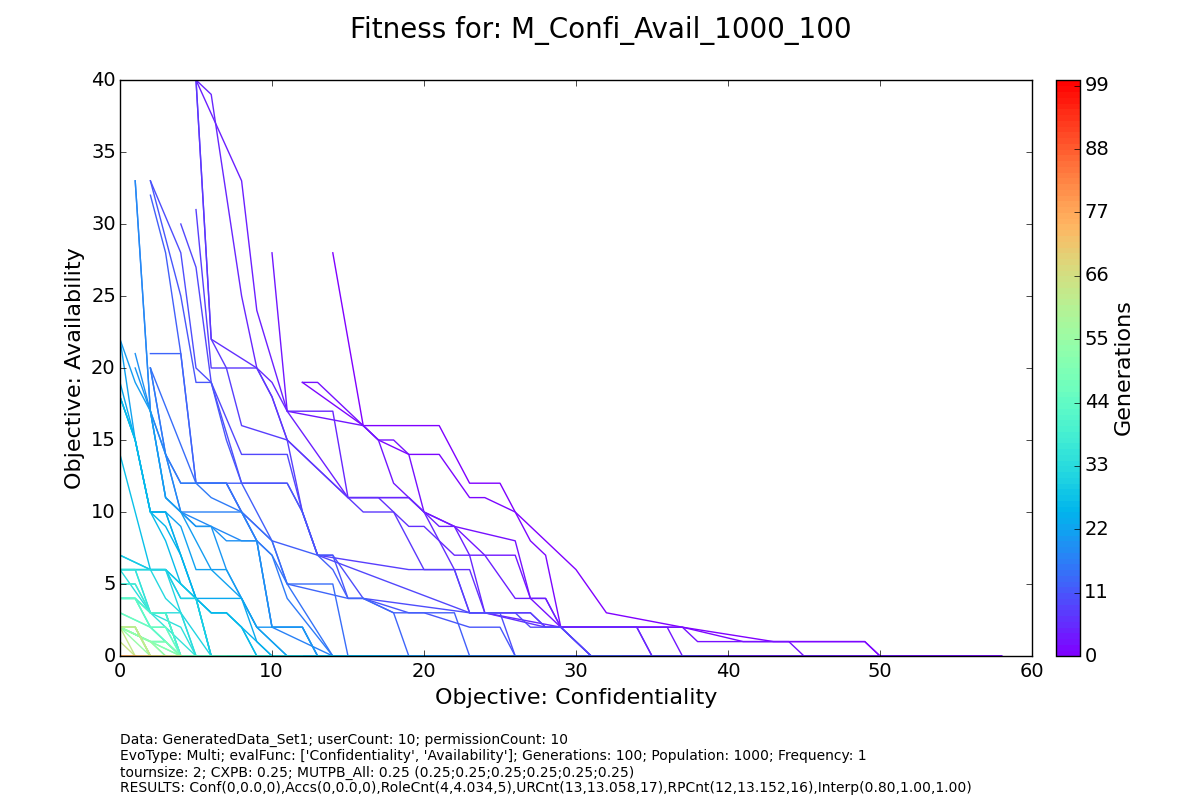
\includegraphics[width=0.8\textwidth, trim=0cm 2cm 0cm 1.5cm, clip=true]{exp4a_fitness_pareto}
		\caption{}
		\label{fig:exp4a_fitness_B}
	\end{subfigure}
	\caption{EXPERIMENT 4a: Example of result of the experiments with Evo-RoleMiner$M$ on Dataset1. (a) Fitness of individuals over several generations (b) Pareto fronts of each generation.}
	\label{fig:exp4a_fitness}
\end{figure}

An example boxplots on the diversity of the role count of individuals of a population is shown in Figure \ref{fig:exp4c_diversity} for the healthcare dataset. Compared to the role count diversity in the experiments with the Evo-RoleMiner (see Figure \ref{fig:exp3c_diversity}), the Evo-RoleMiner$M$ allows more diverse role models with different role count. This is owed to the fact that the confidentiality violation objective tends to prefer less roles, while the availability violation objective can be probably better achieved if more roles are existing (see Experiment 1 in section \ref{sec:exp1}).

\begin{figure}[H]
	\centering
	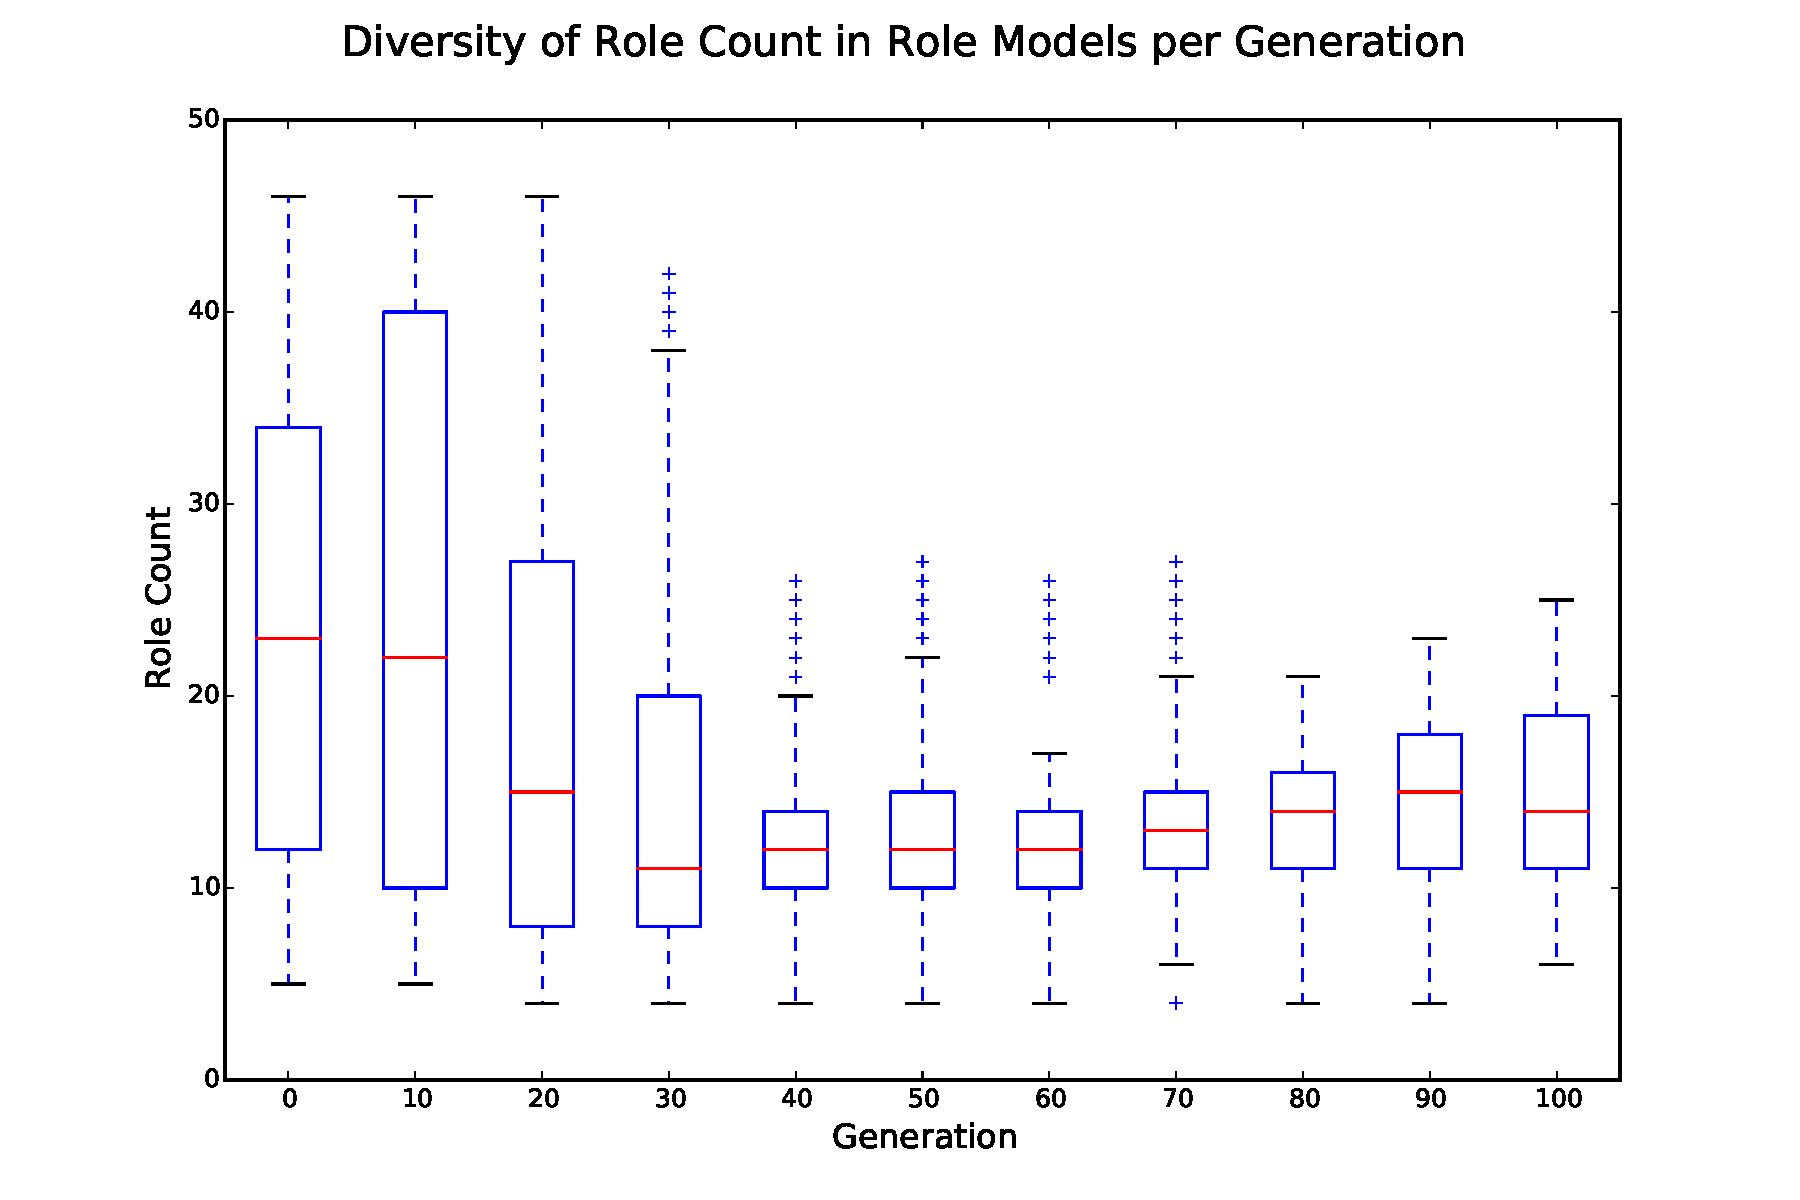
\includegraphics[width=0.7\textwidth]{exp4c_diversity}
	\caption{EXPERIMENT 4c: Example boxplot of role count diversity of individuals of a population in different generations with Evo-RoleMiner$M$ on the healthcare dataset.}
	\label{fig:exp4c_diversity}
\end{figure}

Role models can have the same fitness values for both objectives, although their genotype is different (compare for example the role models in Figure \ref{fig:exp4a_RM_compare}). If several individuals have the same fitness and are in the same non-domination level, they get a crowding distance value of zero (see section \ref{sec:crowdingDistance}). This would imply that role models, who share the same fitness, are favoured in the selection mechanism. Due to this instability in the NSGA-II algorithm, experiment 4b and d are running on a version of the Evo-RoleMiner$M$ based on the improved NSGA-II$R$ algorithm from Fortin et al.\cite{Fortin:2013}. There is a chance that the convergence and diversity of the individuals can be improved, such that the Evo-RoleMiner$M$ can find a solution even faster.

\begin{figure}[H]
	\centering
	\begin{subfigure}[b]{0.5\textwidth}
		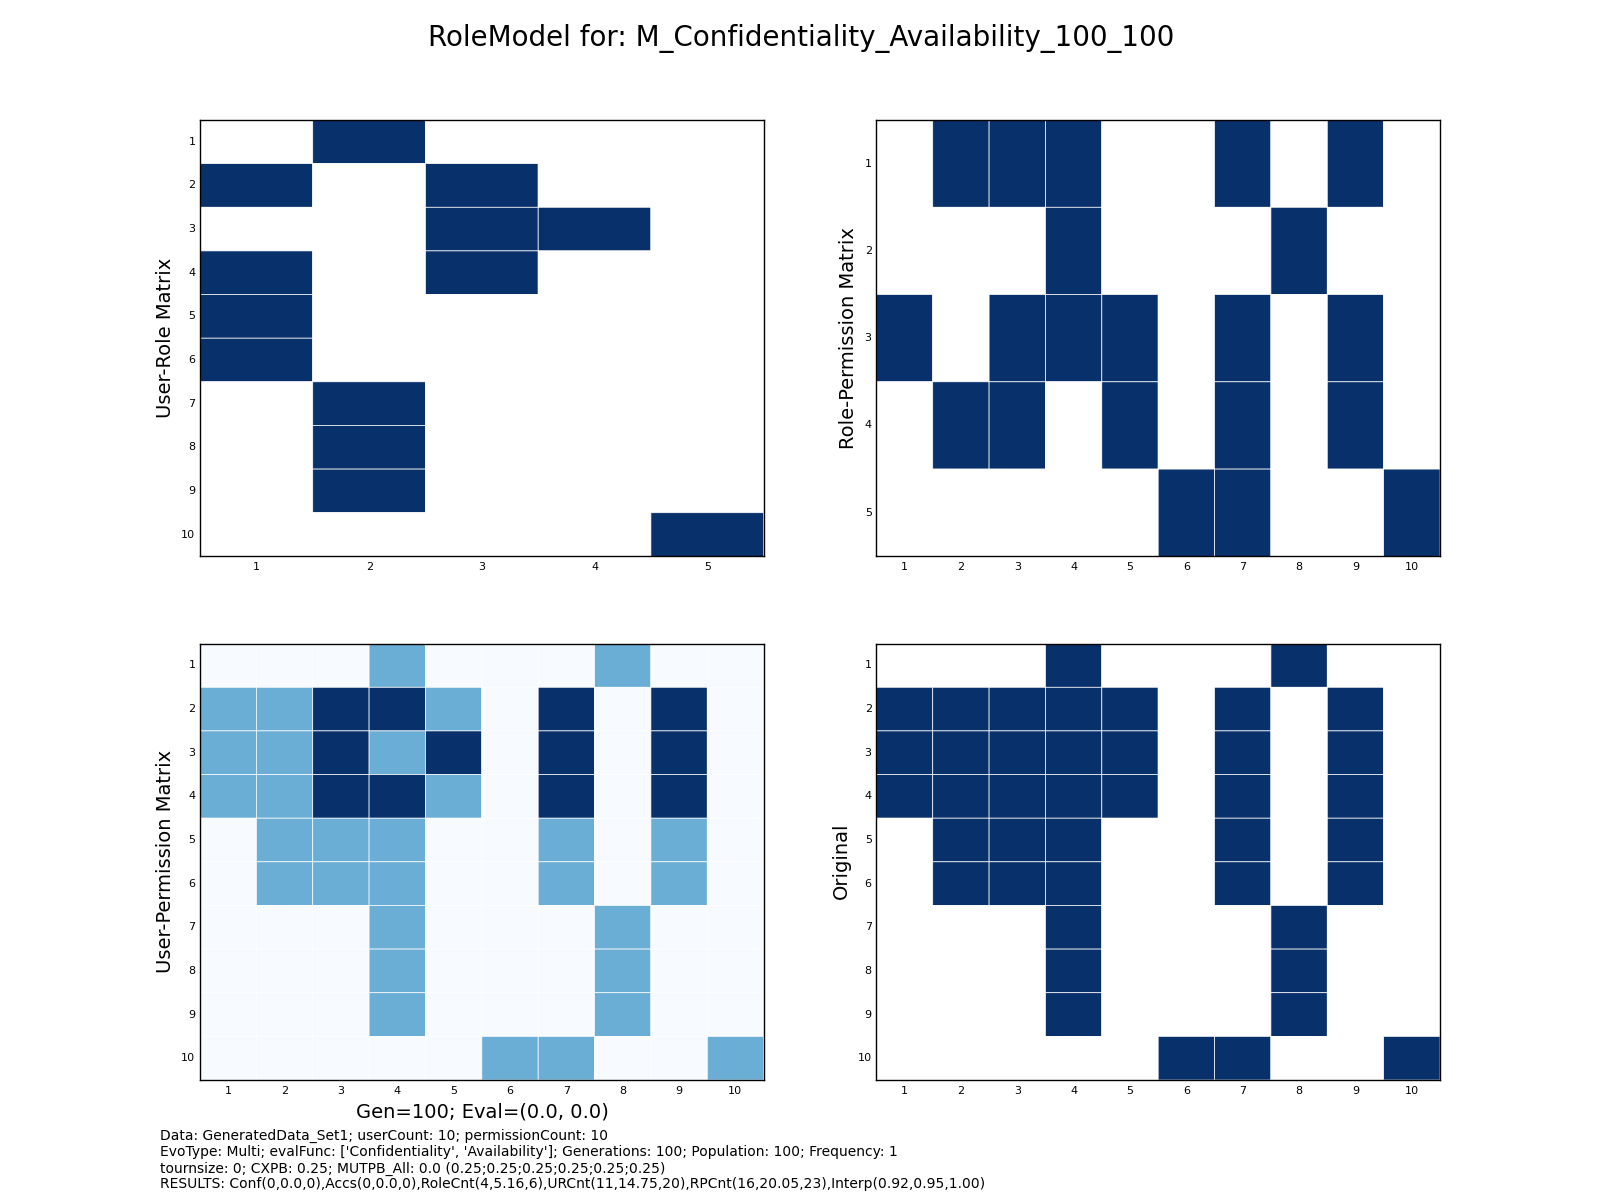
\includegraphics[width=0.9\textwidth,trim=4cm 2cm 4cm 2cm, clip=true]{exp4a_RM}
		\caption{}
		\label{fig:exp4a_RM}
	\end{subfigure}%
	%add desired spacing between images, e. g. ~, \quad, \qquad, \hfill etc. 
	%(or a blank line to force the subfigure onto a new line)
	\begin{subfigure}[b]{0.5\textwidth}
		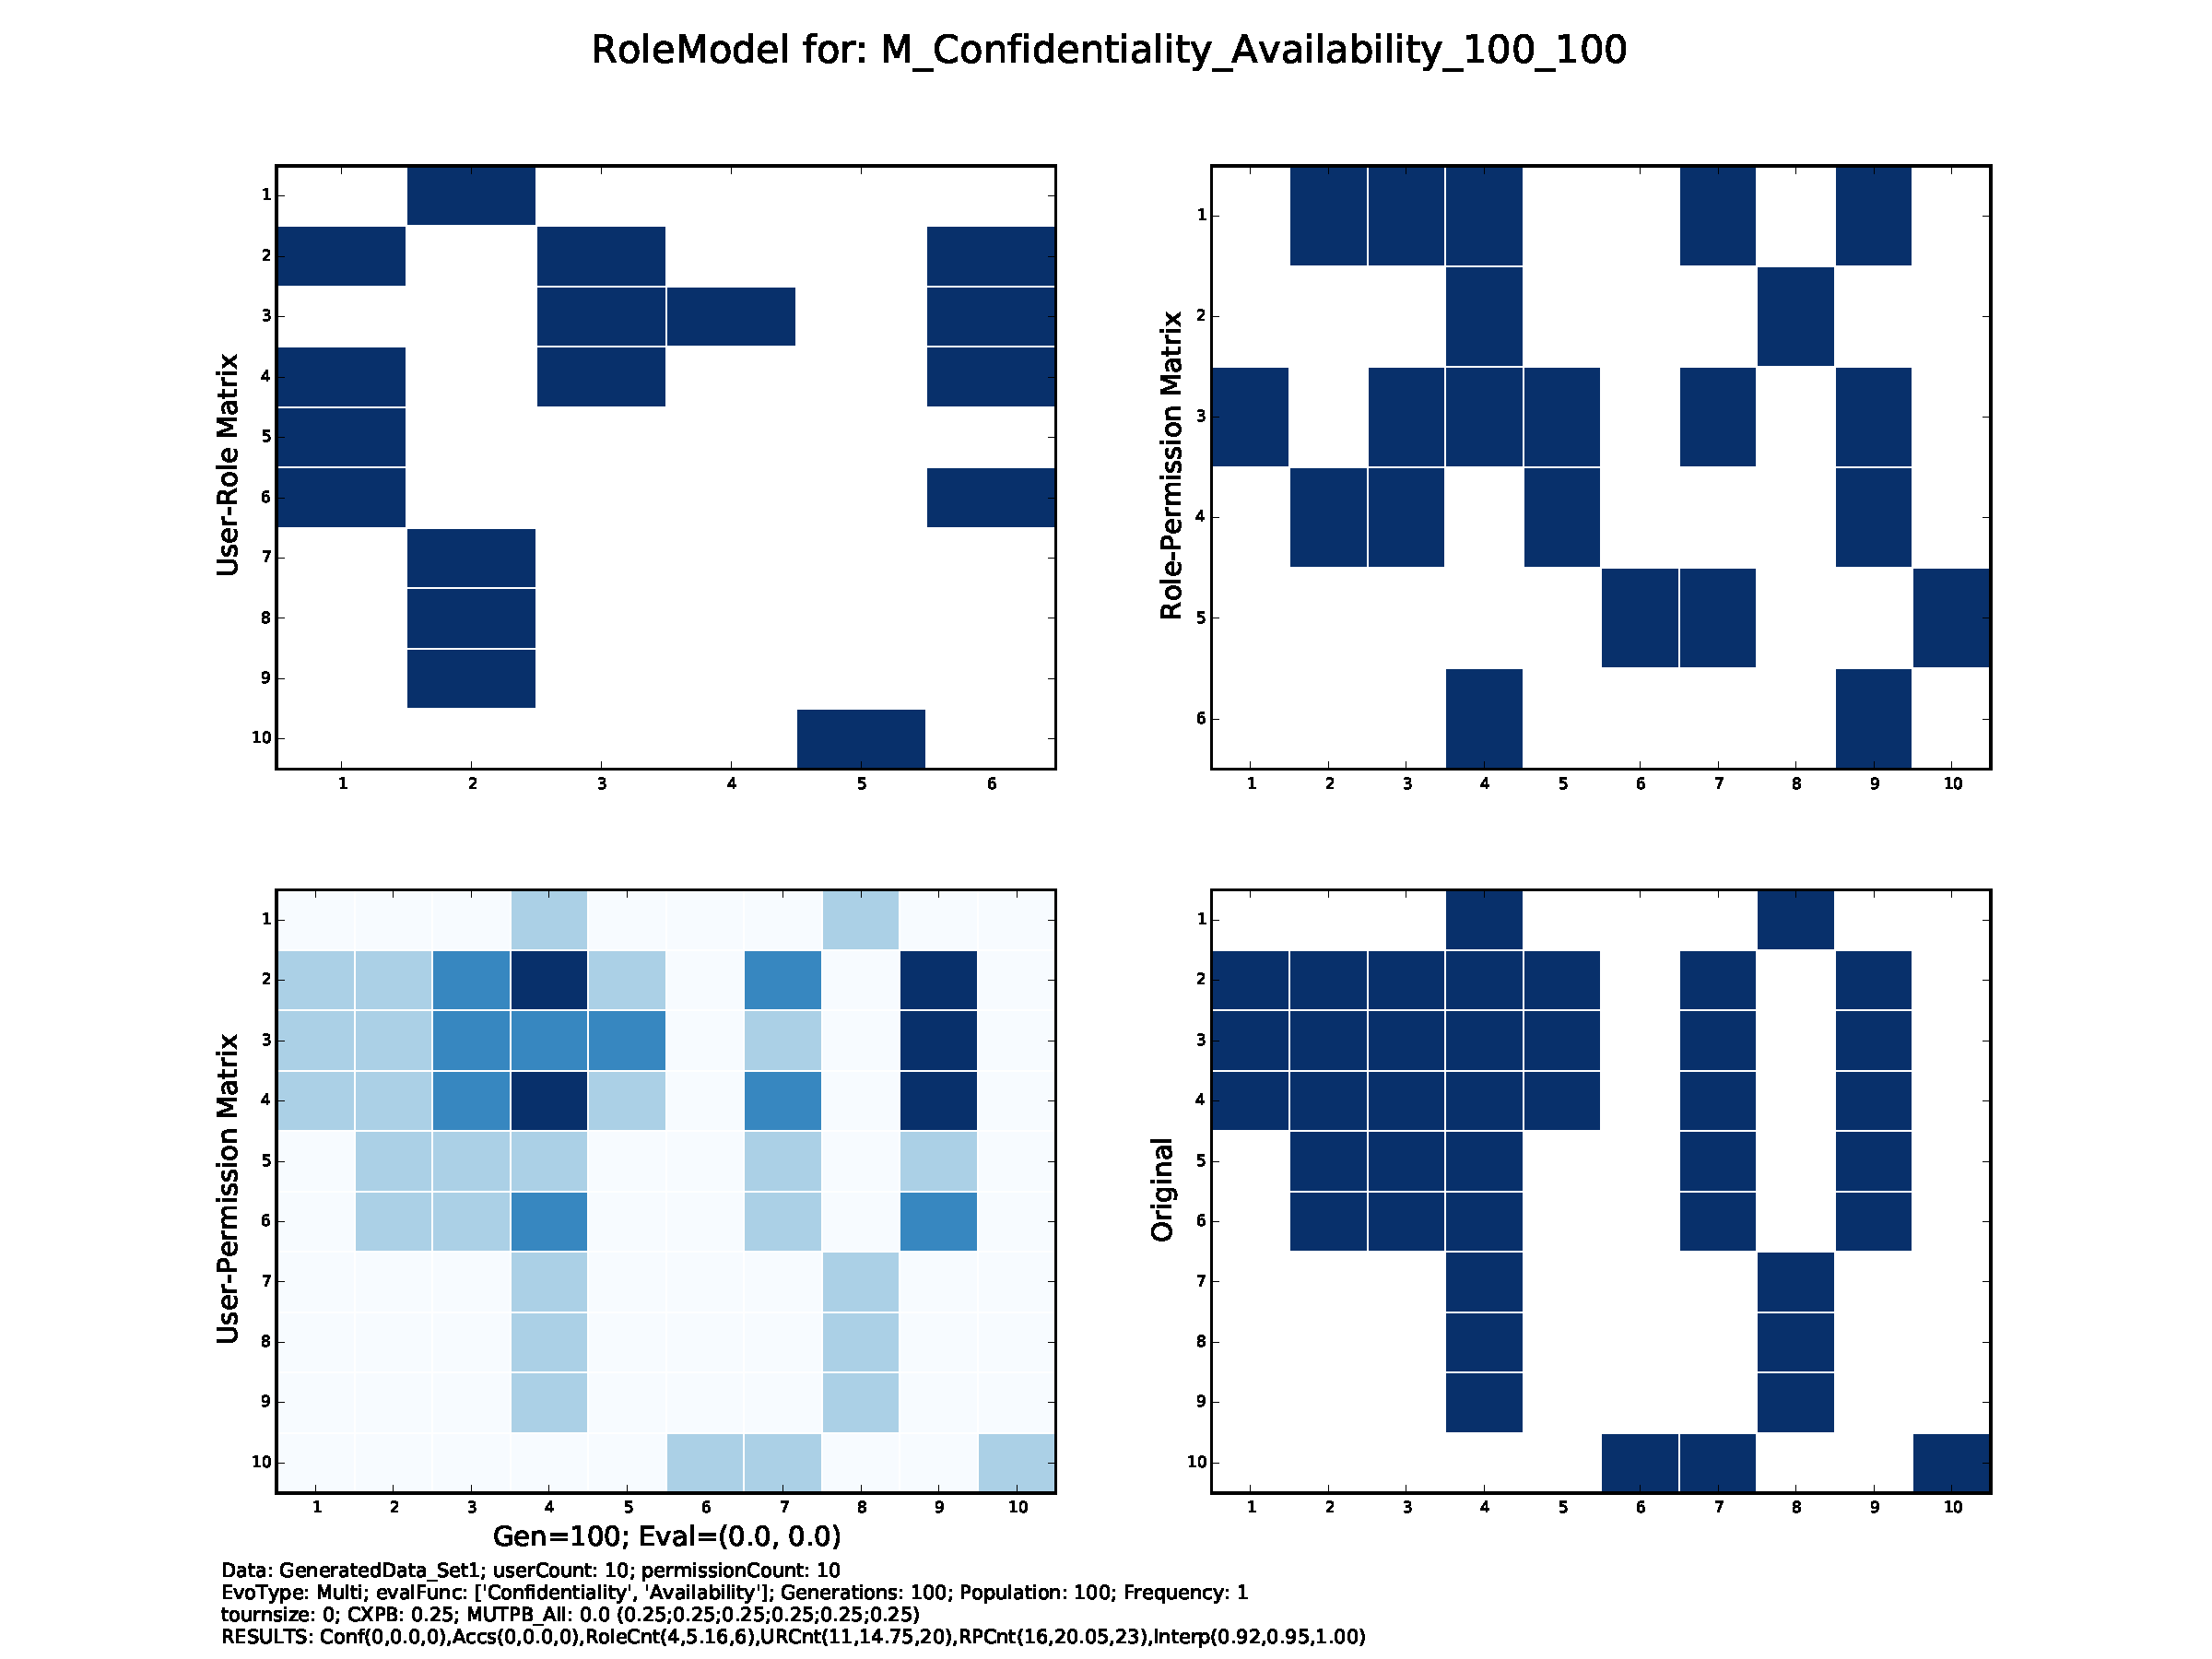
\includegraphics[width=0.9\textwidth, trim=4cm 2cm 4cm 2cm, clip=true]{exp4a_RM2}
		\caption{}
		\label{fig:exp4a_RM2}
	\end{subfigure}
	\caption{EXPERIMENT 4a: Example role models resulting from an experiment on the Evo-RoleMiner$M$ on Dataset1. For each role model from u.l. to l.r.: User-Role Matrix, Role-Permission Matrix, Resulting User-Permission Matrix, Original User-Permission Matrix from Input. A blue box stands for an assignment. The darker the blue the more user-role- and role-permission assignments causing the user-permission assignment.}
	\label{fig:exp4a_RM_compare}
\end{figure}

The results of experiment 4b and d are listed in Table \ref{tab:exp4_results}. In case of experiment 4b it can be seen that the Evo-RoleMiner$M$ based on NSGA-II$R$ gives an improvement, since in average a perfect solution is found after 23.4 generations, while in case of the Evo-RoleMiner$M$ based on the traditional NSGA-II, the average generation when a solution is found is 53 (see experiment 4a in \ref{tab:exp4_results}). Also a T-Test confirmed a statistical significant difference of the generations, when a solution with all objectives fulfilled is found (P-Value=6.379E-10).

The objectives chosen for experiment 4a-d are only confidentiality and availability violations. Although the local optimization is preventing roles with the same user- or permission-assignments, the Evo-RoleMiner$M$ cannot distinguish between the complexity of role models, which can reconstruct the original access policy configuration $UPA$. The Basic RMP optimizes the complexity regards the role count, while the Min-Edge RMP optimizes towards a minimum user- and permission assignment count.

In experiment 4e-f a third version of the Evo-RoleMiner$M$ is tested, where one objective is the minimization of the combined violations count $|G_{conf}^{Min} + G_{accs}^{Min}|$ and the second objective is the minimization of user- and permission assignment count $|UA + PA|$. Since it is known from previous experiments, that the complexity measure has a strong influence the third version of the Evo-RoleMiner$M$ is chosen, which allows to relax the second objective by setting a weight for the second objective (see section \ref{sec:weightedNSGA2}). The weight of the second objective is set to 0.8.

The results can be seen in experiment 4e-f in Table \ref{tab:exp4_results}. In Figure \ref{fig:exp4e_fitness} the development of one of the ten experiments is illustrated. The results show 

\begin{figure}[H]
	\centering
	\begin{subfigure}{\textwidth}
		\centering
		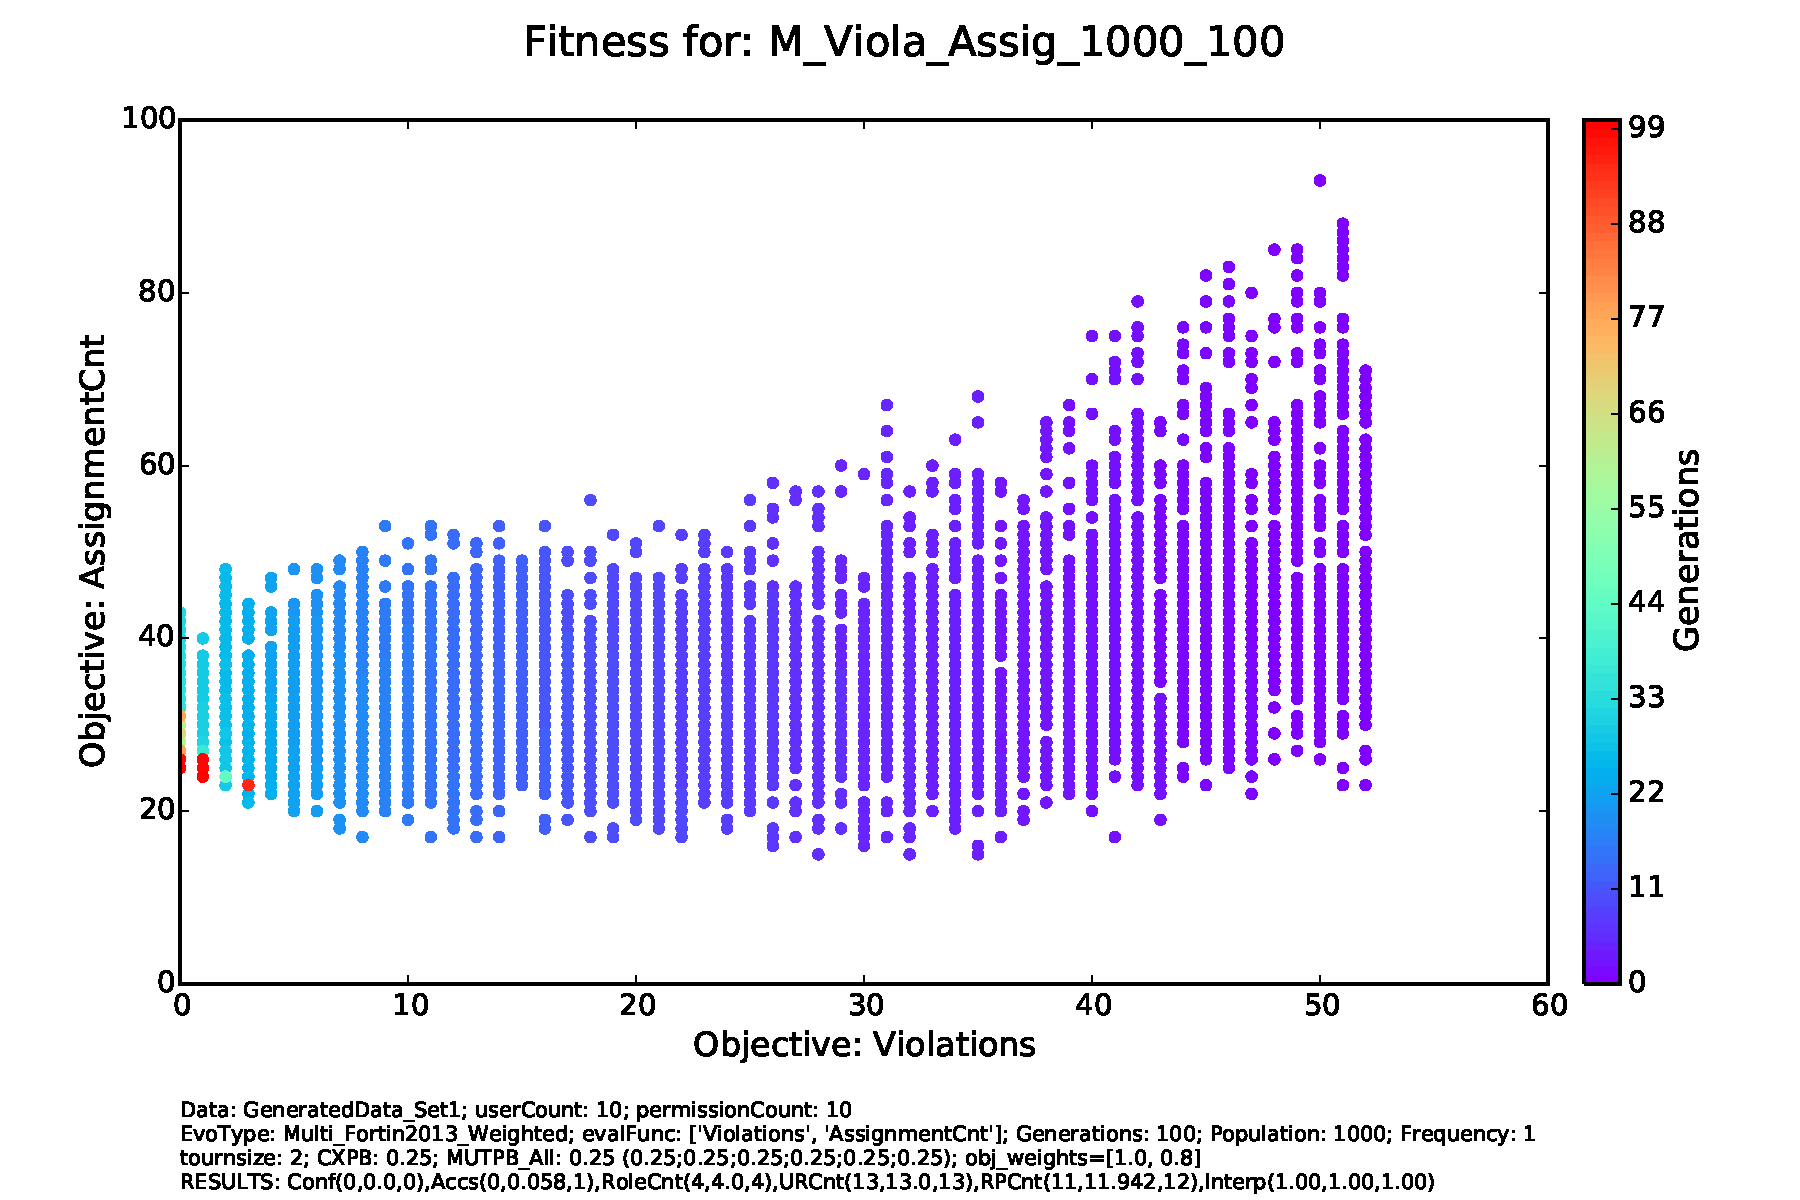
\includegraphics[width=0.8\textwidth, trim=0cm 2cm 0cm 1.5cm, clip=true]{exp4e_fitness}
		\caption{}
		\label{fig:exp4e_fitness_A}
	\end{subfigure}
	\begin{subfigure}{\textwidth}
		\centering
		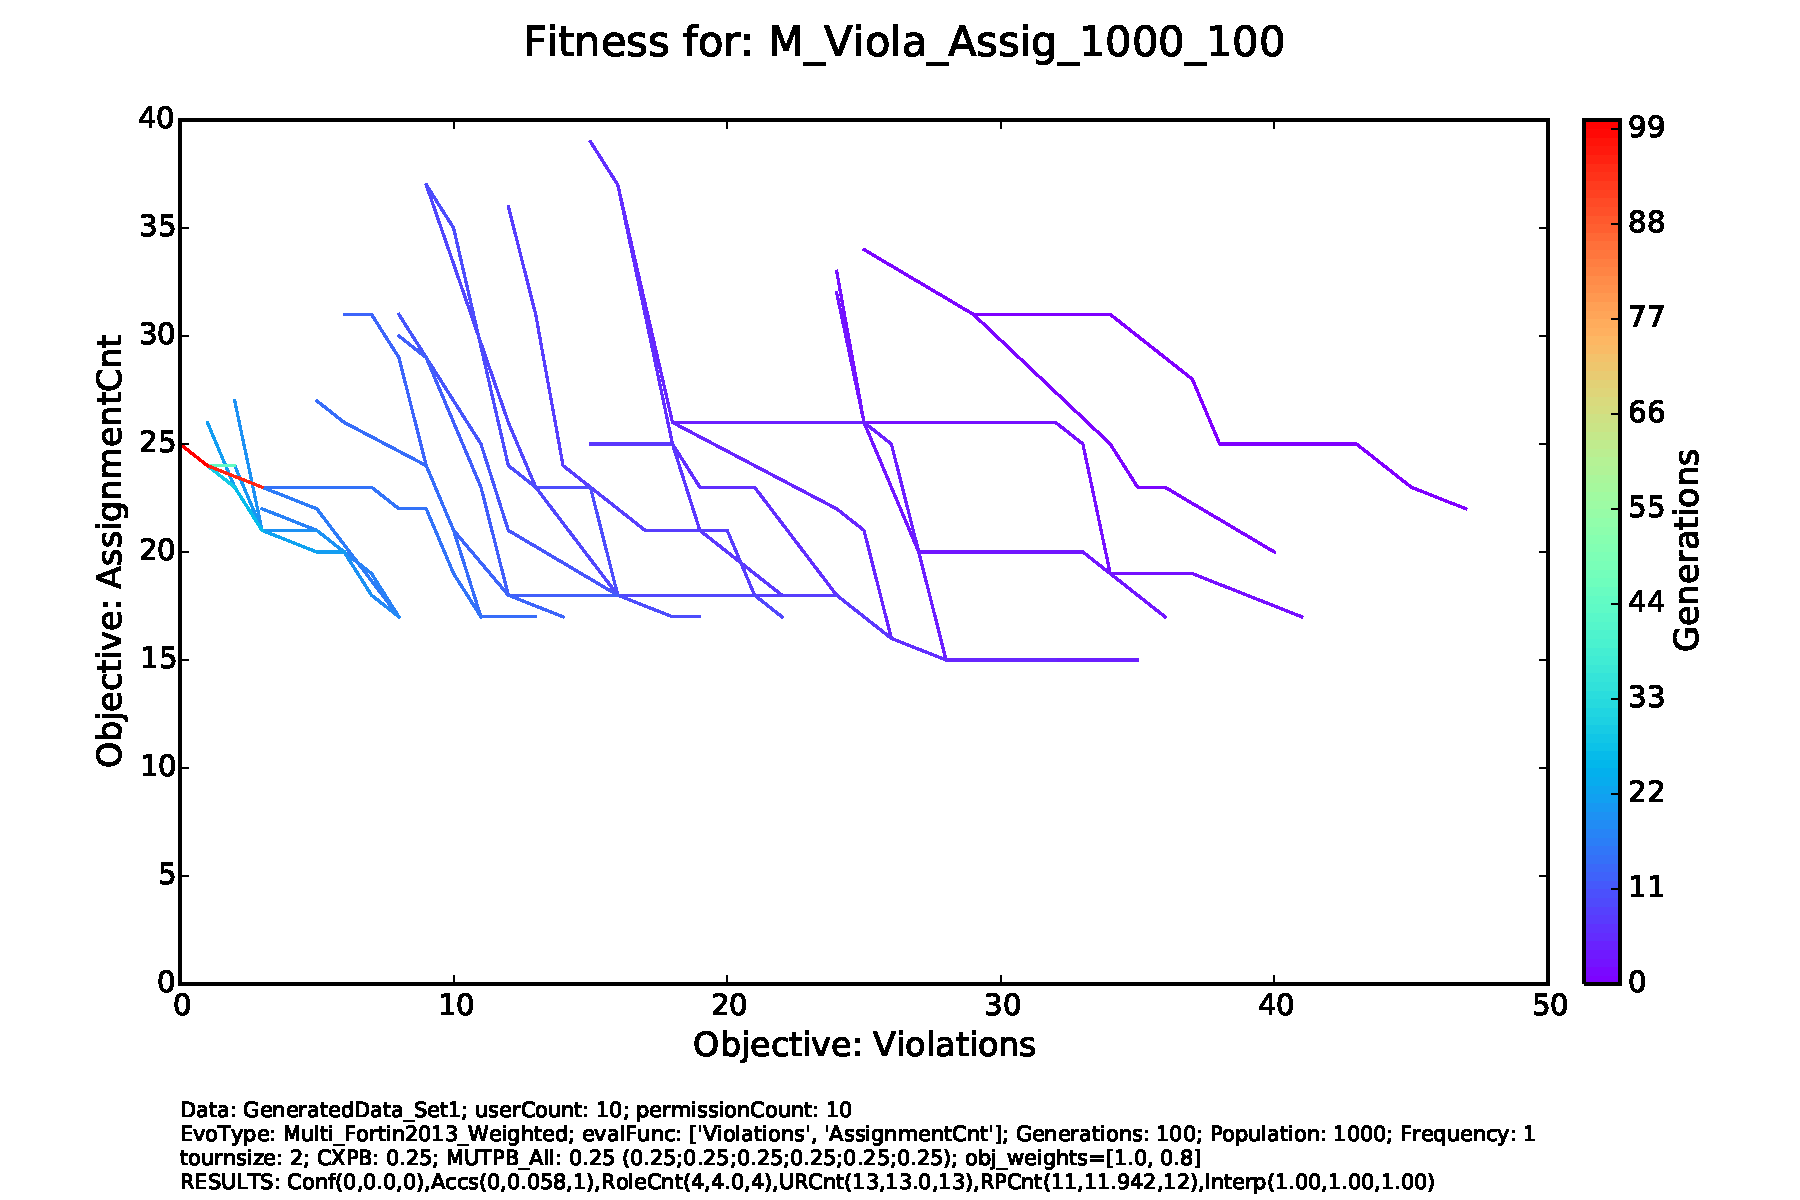
\includegraphics[width=0.8\textwidth, trim=0cm 2cm 0cm 1.5cm, clip=true]{exp4e_fitness_pareto}
		\caption{}
		\label{fig:exp4e_fitness_B}
	\end{subfigure}
	\caption{EXPERIMENT 4e: Example of result of the experiments with Evo-RoleMiner$M$ version 3 on Dataset1. (a) Fitness of individuals over several generations (b) Pareto fronts of each generation.}
	\label{fig:exp4e_fitness}
\end{figure}



